\section{Optimisation of Investment Strategies}

Most usually, classical savings theory states that the optimal approach to ensure the risk level of any given investment is to set a constant proportion of the wealth allocated in risky assets.

In this section we will explain how we simulate the result of such strategies and compare them to the methodology of the work developed in \cite{a:guillen-optimisation}, in which they explain the idea of a \emph{variable} proportion allocated in risky assets, instead of constant. We will replicate the results of that work and see how this change in the strategy can affect the performance of the investment plan.

\subsection{CPPI Scheme}

Firstly, we will start defining the \textit{benchmark} model. The constant portfolio strategy follows the logic derived from constant relative risk exposure.

This methodology consists in investing a constant proportion $\pi$ of the savings in risky assets (subject to volatility), whilst investing the rest $1 - \pi$ in risk-free assets. Thus, the time evolution of the wealth $X$ of an investor would behave as following:

\begin{align}
	dX = \alpha \pi X(t)dt + \sigma \pi X(t)dW(t) + dC(t)\textit{.}
\end{align}

Where $\alpha$ is the expected return of the risky market, $\sigma$ is the expected volatility of the risky market, $W(t)$ is a Wiener process and $C(t)$ is the allocated or consumed capital by the investor at every time step.

The point of this strategy is to present an intuitive straightforward way to control the risk exposure in savings strategies. The simplicity of this approach let us tweak $\pi$ in order to make the investment best suited for the risk aversion profile of each investor individually.

\subsection*{Simulation}

In order to simulate the performance of this kind of strategy, we start assuming that the risky assets follow a simplified geometric brownian motion, with \emph{trend} $\alpha$ and \emph{volatility} $\sigma$. Thus, if the saver invests $x$ in this asset at day $t$, the wealth of the saver at the next day would be $x_{t+1} = (1 + N\qty(\alpha, \sigma)) x_t$.

This way, we construct the scenario of an investor, saving a fixed amount of money - which is denoted as $a$ -   throughout $T/2$ years. That money being allocated $( 1 - \pi) a$ in the risk-free asset, which we will set with return 0; and $\pi a$ allocated in the risky asset, whose expected return is $\alpha$ and volatility is $\sigma$. Thus, if we set $x_t$ as the wealth at any given time $t$, we can see that

\begin{align}
	x_{t+1} = (1+N(\alpha, \sigma))x_{t}\pi + (1 - \pi)x_{t} + a \textit{.}
\end{align}

At some point in time, our investor will stop saving money and will start consuming it (as in most pension plans), so we just convert that fixed amount of money $a$ to \emph{consumed} money instead of saved. Thus, the evolution of wealth turns out to be:

\begin{align}
	x_{t+1} = x_{t}(1+N(\alpha, \sigma))\pi + (1 - \pi)x_{t} - a \textit{.}
\end{align}

At the end of all $T$ years, the final wealth $X_T$ remaining to the saver is stored. By reproducing this same scheme, we manage to compute tens of thousands of different performances and make some statistics out of them.

\begin{figure}[H]
    \centering
    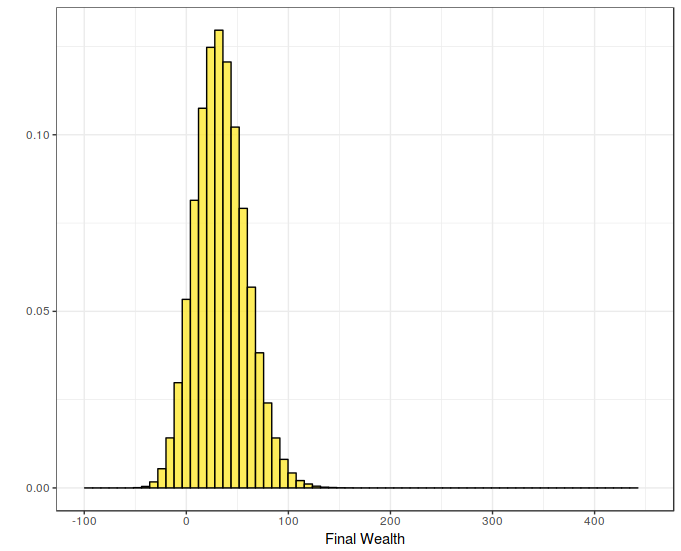
\includegraphics[scale=0.65]{./images/fw_cppi.png}
    \caption{Results of the simulation for the CPPI model. Final wealth obtained for every simulation, over $10,000$ simulations, where $T=60$, $\mu = 0.0343$, $\sigma = 0.1544$, $a=10$, $\pi = 0.1$}
    \label{fig:cppi_fw}
\end{figure}

The first impression we get when looking at the histogram from Figure\ref{fig:cppi_fw}, is that it has the shape of a \textit{Bell Curve}, thus following a \textit{Normal Distribution} It seems quite symmetric and is slightly skewed towards positive results, what would imply modest positive results at the end of the plan.


The code necessary to replicate these results in R can be found in Appendix \ref{ap:cppi-simple}
